\section{Nature-inspired computing}

\textbf{1. Describe the main components of an evolutionary program:
population representation, generation, selection, combination,
replacement, and stopping criteria?}

Represent the population with a list of solutions, start with a randomly
generated or systematically built population. Compare solutions to each
other using a fitness function to evaluate them. Select the best ones to
combine them into new solutions (crossover), mutate some to get a new
random solution that can expand the search space.

Stopping criteria: n generations, when no change in top x for n
iterations, when no change in population for n iterations, resources
(time), target fitness.


\textbf{2. Describe when to use genetic algorithms?}

GAs are good, when there is a clear way to evaluate fitness of solutions
(and we don't know the original function - if we would, you don't need
GA for it), when we have a big space to search and when we can find a
good representation of genes (agents). For example we can use them with
TSP where a fitness function is the distance of the traversed path.

\textbf{3. Describe the strengths and weaknesses of evolutionary
programs.}

Strengths: robust, adaptable and general, requires only fitness function
and representation of genes

Weaknesses: can get stuck in local extreme, can take a long time to
converge to solution, time complexity rises fast with bigger population

\textbf{4. Describe the main characteristics of genetic algorithms (GA)
and genetic programming (GP).}

GA is based on evolution. $\rightarrow$ I think the same answer as in
1. Applies here

GP instead of representing solutions in list/objects, represent them
with tree structures. Crossover: exchange subtree, mutation: random
change in trees. Variable length encoding, more flexible, often grow in
complexity

\textbf{5. Describe terms from evolutionary computation such as
population variability, fitness function, coevolution.}

\textit{Fitness function}: is a function that takes a solution as
input and evaluates it, to see how ``good'' the solution is.

\textit{Population variability}: we need to have a population that
encompasses as big a solution space as possible to find a solution close
to the optimal as possible (eg. 2\^{}30 solution space, population of 10
will probably not find a very good solution)

\textit{Coevolution}: basically crossover $\rightarrow$ two agents
affect evolution by combining traits.

Was mentioned more in context of solving related problems together

\textbf{6. Describe different gene representations in GA, operations on
them, and their strengths and weaknesses: bit and numeric vectors,
strings, permutations, trees.}

\textit{bit/numeric:} good for problems that can be represented with
numbers, cannot represent very complex problems, eg. good for knapsack
problem

\textit{Strings:}

\textit{Permutations}: good for problems where we are looking for a
solution of a sequence of numbers (TSP), then we can use GA to ``learn''
the best permutations

\textit{Trees}: good for problems where we want to find the formula
for the solution (as formulas can be nicely represented with trees)

\textbf{7. What are linear crossover, Gray coding of binary numbers,
adaptive crossover, gaussian mutation, Lamarckian mutation, and elitism?
What are their advantages compared to baselines?}

\textit{Linear crossover:} takes a linear combination of the two
individuals, have a ``probability'' for each bit in each agent and take
each bit with probability p from agent 1 and with probability (1-p) from
agent 2

\textit{Gray coding:} Encode binary numbers in such a way that
incrementing a number by 1 takes only 1 bit change (Sth like this: Order
binary representations of numbers in such a way that the next number is
only one bit changed: 0 - 1 - 11 - 10 - 110 - ...)

\textit{Adaptive crossover:} Use bit templates for crossover (1-first
parent, 0-second parent). Learn which templates work best

\textit{Gaussian mutation:} Mutate by adding a Gaussian error to the
mutation

\textit{Lamarckian mutation:} search for locally best mutation

\textit{Elitism:} choose n of the best solutions in population and
keep them for the next population

\textbf{8. Describe the following evolutionary models: proportional and
rank proportional roulette wheel, tournaments, single tournament, and
stochastic universal sampling?}

\textit{Tournaments:} have agents ``battle'' each other, by assigning
them probabilities according to their fitness values. Best solution
$\rightarrow$ best probability of winning.

\textit{Proportional:} Assign each agent a probability according to
their fitness value. Use randomly generated numbers to select agents.

\textit{Rank proportional:} Assign each agent probability according
to their rank of fitness value.

\textit{Single tournament:} randomly split population into small
groups and apply crossover to two best agents from each group, their
offspring replace the two worst agents from the group

\textit{Stochastic:} F = sum(all fitness values), N = size of
population we want. Make a F/N interval. Assign part of the interval to
each agent according to fitness values. Use RNG to generate numbers, if
generated number is within an interval of some agent $\rightarrow$
choose the agent

\textbf{9. How to prevent niche specialization in GA?}

We punish agents that are too similar to others $\rightarrow$
depending on the type of problem (min/max) decrease/increase the fitness
value

\textbf{10. Explain hypotheses on why GAs work?}

When we have a big enough population and the right parameters, we can
search a pretty big solution space.

\textbf{11. What are the typical parameters of GAs?}

Probability of crossover, probability of mutation, population size, max
number of iterations, max number of iterations with the same best
solution, selection method, termination criteria.

\textbf{12. Where to use GAs and where not?}

YES: where there are many local extrema, fitness function easily
defined, robustness, don't need specialized methods

NO: huge solution spaces with large solutions (eg. list of list of list)

\textbf{13. Why are GAs suitable for multiobjective optimization, and
what is Pareto optimal solution?}

Use fitness functions with different objectives and try to improve them.

\textit{Pareto}: we cannot improve conflicting criteria without
getting worse on others

\textbf{14. Explain the main problems of genetic programming.}

Needs huge populations(thousands), it's slow, problems involving
physical environments: making trees that are really executable,
execution can change the environment which changes fitness function,
calculating fitness function with simulation takes a lot of time.

\section{Machine learning}

Try to estimate $f(X)$ so we can get the most accurate $Y$ to the actual
result.

\[ Y = f(X) + \varepsilon\]

\textbf{15. Describe the two main goals of ML, prediction and inference,
and explain why they are sometimes in contradiction.}

\textit{Prediction}: if we can make a good estimate, then we can make
accurate predictions for the response $Y$ based on $X$

\textit{Inference:} we are interested in the type of relationship
between $Y$ and $X$, model interpretability is essential for inference.

If we want good accuracy (prediction), we might need a much more
complicated model which will have lower interpretability and vice versa.
But it can also happen that some complicated model gives us bad results
(overfitting) and thus lower accuracy.

\textbf{16. What parametric and non-parametric ML methods exist?}

\textit{Parametric methods}: Logistic regression, Naive bayes, simple
neural networks

\textit{Non-parametric methods}: kNN, decision trees, SVM

\textbf{17. Describe the main characteristics of supervised,
unsupervised, and semi-supervised ML methods?}

\textit{Supervised learning:} both $X$ and $Y$ are observed

\textit{Unsupervised:} only $X$ are observed, we need to use $X$ to guess
what $Y$ would have been and build a model from there

\textit{Semi-supervised}: only a small sample of labelled instances
are observed but a large set of unlabeled instances

\textbf{18. What is the difference between regression and
classification? Give examples of problems for each type.}

Regression: $Y$ is continuous/numerical (predict the value of a share on
the stock market, predict the temperature).

Classification: $Y$ is categorical (predict if an event will happen, eg.
is this email spam or not, will it be cloudy, rainy or sunny)

\textbf{19. What are association rules, and how they differ from
decision rules?}

\textit{Association rules} are rules that tell us how some ``event''
is associated with another (how some $X$ is associated with some $Y$).

\textit{A decision rule} is a simple IF-THEN statement consisting of
a condition and a prediction.

\textbf{20. What are outliers in ML?}

A data object that does not comply with the general behavior of the
data. It can be noise or an exception.

\textbf{21. Contrast two different views on ML: as optimization and as
search.}

Usually the goal of classification is to minimize the test error.
Therefore, many learning algorithms solve optimization problems.

Optimization: objective is to minimize test error (optimize cost
function)

Search: find parameters that describe our $f(X) = y$ best

\textbf{22. Describe different properties of ML models: bias, variance,
generalization, hypothesis language.}

\textit{Bias} refers to the error that is introduced by modeling a
real life problem by a much simpler problem. The more flexible/complex a
method is, the \textbf{less} bias it will have

\textit{Variance} refers to how much your estimate for f would change
if you had a different training data set. The more flexible the method
is, the \textbf{more} variance it has.

\textit{Generalization} describes how well our method works on new
unseen data (aka test data).

\textit{Hypothesis language} describes the hypotheses which machine
learning system outputs

\textbf{23. What is the bias-variance trade-off in ML?}

If we have too much bias, we won't have a lot of variance giving us a
very inflexible method that doesn't predict well. If we have too much
variance, the model could overfit to the training data and will not work
well with new unseen data. In both cases the error of prediction will be
high, so we want to find that sweet spot where we minimize the error
rate, but don't overfit.

\textbf{24. Describe the double descent concerning bias-variance
trade-off.}

For every model there is a spot in how much data we use that will have a
very bad error rate. (eg. a model can predict well on the test and train
set for 5000 samples and predict very poorly for 7500, but predict very
well for 10000 again)

This is observed only in neural networks (and random forests(?)). Other
models observe the ``classic'' overfitting phenomenon.

% 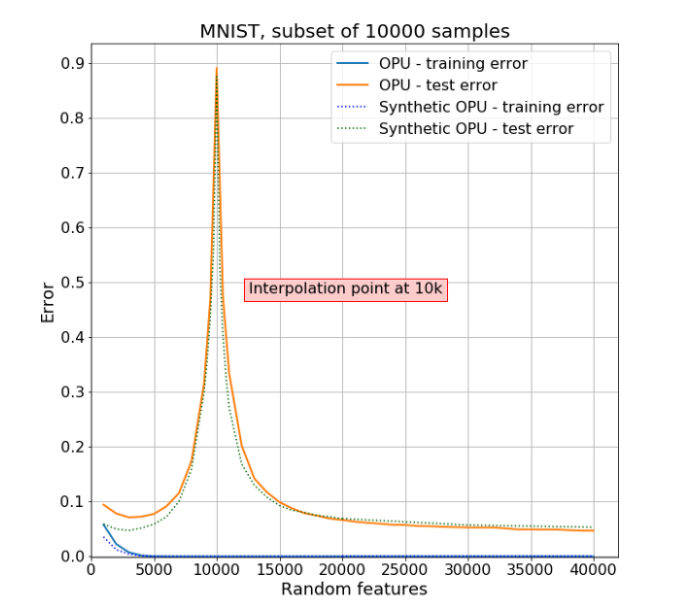
\includegraphics[width=\columnwidth]{media/image1.png}

When model complexity keeps increasing, the testing error first starts
decreasing due to the adaptation of model parameters to the data
features. After the sweet spot that is proposed by the classical wisdom,
testing error starts rising and generalization keeps worsening. However,
after the complexity exceeds the interpolation threshold, the mystery
happens. As long as we keep increasing the model complexity, test error
keep decreasing and after certain complexity, the testing error start to
be smaller than the sweet pot that we get within the
\textit{under-parameterization regime}

% 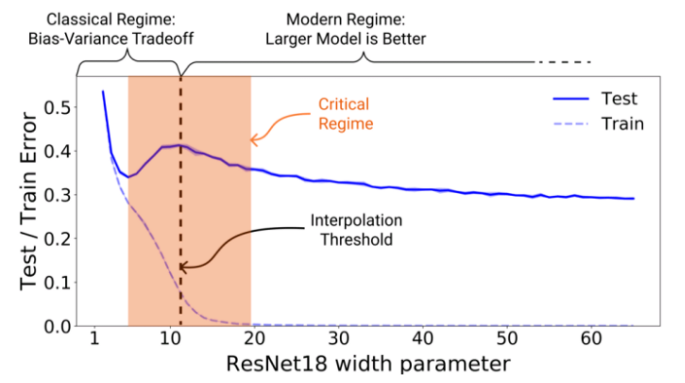
\includegraphics[width=\columnwidth]{media/image24.png}

\textbf{25. Describe bias-variance trade-off in relation to kNN
classifier.}

Variance generally decreases with increasing k, bias increases with
increasing k

\textbf{26. Describe methods that can speed-up the kNN algorithm: k-d
trees, R-trees, RKD-tree, locally sensitive hashing, and hierarchical
k-means.}

\begin{itemize}
\item \textit{k-d} trees are a generalization of BST, where each node
  holds a vector instead of a single value. Before building a tree we
  must normalize values to the interval {[}0,1{]}, and we split each
  node on dimension so that we maximize variance in that dimension, and
  we use the median of that dimension as a splitting value. Leaves
  usually hold multiple values.
\item \textit{R-trees} are similar to k-d trees but are generalization of
  B-trees.
\item \textit{RKD-trees} are multiple trees where we split on random
  dimensions from a set of dimensions with highest variance. If the
  probability of not finding nearest neighbor in the single tree is p
  then with m trees is p\^{}m
\item \textit{Local sensitive hashing}: we have multiple hash tables with
  multiple hash functions, near instances are also near when hashed
  (hashing with random hyperplanes)
\item \textit{Hierarchical k-means}: recursively run k-means clustering,
  until clusters are small enough
\end{itemize}

\textbf{27. What are the Bayes error rate and Bayes optimal classifier?}

Bayes error rate refers to the lowest possible error rate that could be
achieved if somehow we knew exactly what the ``true'' probability
distribution of the data looked like.

Bayes optimal classifier for new x0 returns the maximally probable
prediction value P(Y=y\textbar X=x0)

\textbf{28. Describe properties of the following models: kNN, decision
rules, bagging, boosting, random forests, stacking, AODE, MARS, SVM,
neural networks.}

\textit{kNN:} represent the data in a 2D/3D\ldots{} space and compute
distances between different data samples, use these distances to find
the k nearest neighbors to our input x0 and classify x0 as the majority
class of these k instances.

\textit{Decision rules}: is a function which maps an observation to
an appropriate action.

\textit{Bagging:} make different bags for each classifier and put
data samples in them, classify new data sample by comparing it to the
samples in the bags

\textit{Boosting}: grows tree sequentially $\rightarrow$ each tree
uses information about errors of previous trees, weak learners ensemble

\textit{Random forests}: build an number of decision trees on
bootstrapped training sample, but when building these trees, each time a
split in a tree is considered, a random sample of m predictors is chosen
as split candidates form the full set of p
predictors

\textit{Stacking:} Predictions of base learners are used as input for
meta learner (shitty neural networks).

Method to combine heterogeneous predictors.

Predictions of base learners are used as input for meta learner.

\textit{MARS}: Multivariate Adaptive Regression Splines

Generalization of stepwise Linear regression.

Not tree-based. Adds one variable at the time (sees which 1 is the
best).

It is a
\href{https://en.wikipedia.org/wiki/Non-parametric_regression}{non-parametric
regression} technique and can be seen as an extension of
\href{https://en.wikipedia.org/wiki/Linear_model}{linear models} that
automatically models nonlinearities and interactions between variables.

\textit{AODE:} Average One-Dependence Estimator

ensemble of SPODE classifiers (Super-Parent One Dependence Estimator --
Naive Bayes where attributes are dependent on class and one more
attribute).

All attributes in turn are used in SPODE classifier and their results
are averaged

It has higher variance but lower bias than Naive bayes.

\textbf{Averaged one-dependence estimators} (\textbf{AODE}) is a
probabilistic
\href{https://en.wikipedia.org/wiki/Classifier_(mathematics)}{classification
learning} technique. It was developed to address the
attribute-independence problem of the naive bayes classifier.

\textit{SVM:} Support Vector Machine $\rightarrow$ constructs a
hyperplane or set of hyperplanes in a high dimensional space which can
be used for classification or regression.

\textit{Neural networks}: use layers of neurons to compute the
result, neurons are connected with edges that have weights, these
weights are used to represent the importance of one neuron's output for
another neuron's input. Use backpropagation to learn these weights.

\textbf{29. What is the difference between training and testing error?
Why do we need an evaluation set?}

Training error is the error rate we get on training data, testing error
is the error we get on the test data. Mostly if training error is very
low, the model will overfit, which will produce a high testing error and
a badly generalized model.

We need the evaluation set to test our model on previously unseen data
and see if we overfitted it.

\textbf{30. Describe the properties and purpose of evaluation with
cross-validation. Describe different biases of ML models stemming from
data: reporting bias, automation bias, selection bias, group attribution
bias, implicit bias.}

\textit{Cross-validation}: when we don't have enough data to split
(or we don't want to split), we make k splits and build a model for each
subset and test it on remaining data. Every instance is used for testing
once and we get a general idea of model accuracy on that data.

\textit{Reporting bias:} frequency of data is not real world
frequency (people review only if they have extreme opinions \ldots)

\textit{Automation bias:} model is actually not better than human
performance (but you love ML and you want to use it \ldots)

\textit{Selection bias:} data sets are not representatively selected
(interview only friends and family, even selecting complete strangers we
have some bias in selection)

\textit{Group attribution bias:} is a tendency to generalize what is
true of individuals to an entire group to which they belong. (you went
to FRI and generalize that all are good students \ldots{} )

\textit{Implicit bias:} occurs when assumptions are made based on
one's own mental models and

personal experiences that do not necessarily apply more generally. (i
think, so it must be true)

\textbf{31. What is the no-free-lunch theorem?}

No universal algorithm is the best algorithm. (we cannot say SVM is
better than RF, we cannot mathematically prove that)

There cannot be a single best algorithm for every ML situation.

\textbf{32. Describe three types of feature selection methods: filter,
wrapper, and embedded methods. What are the main differences between
them?}

\textit{Filter methods}: independent of learning algorithm, select
the most discriminative features through a criterion based on the
character of data (information gain, ReliefF)

\textit{Wrapper:} use the intended learning algorithm to evaluate the
features (eg. progressively add features to SVM while performance
increases)

\textit{Embedded}: select features in the process of learning (ridge,
lasso)

\textbf{33. Describe the difference between impurity based and
context-sensitive attribute evaluation.}

\textit{Impurity based}: assume \textit{conditional independence
between the attributes} (information gain, Gini index, MDL, distance
measure, MSE, MAE (mean absolute error))

\textit{Context sensitive measures:} contrary (Relief, Contextual
Merit). Random forest or boosting based attribute evaluation.

\textbf{34. Describe the main ideas of information gain and ReliefF
evaluation measure.}

\textit{Information gain}: measure (im)purity (entropy) of labels
before and after the split

IG(A) = H(T) - H(T\textbar A).\\
H \ldots{} Information entropy

H(T\textbar A) \ldots{} conditional entropy

Assumes attributes are independent.

\textit{ReliefF:} criterion: evaluate attribute according to its
power of separation between near instances. Increases/decreases worth of
feature(s) when comparing the (dis)similarity between random nearby
examples (based on certain attribute). Nearest k hits.

\textbf{35. Explain how regularization can be used as a feature
selection method?}

(Regularization is a technique used to reduce the errors by fitting the
function appropriately on the given training set and avoid overfitting.)

Example → Lasso (L1) regression \ldots{} attributes (parameters in
linear regression) will be set to 0 if they are useless \ldots{}

\textbf{36. Describe ridge regression (L2) and lasso (L1) and the
difference between them?}

The key difference between them is the penalty term.

\textit{Lasso → L1} type regularization, which means that it does not
square the size of the attribute parameter. It only sums up the sizes
and adds it to the error estimation. It will automatically converge
these parameters to zero, if they don't contribute to the prediction.

In other words, if the parameter does not contribute to the prediction,
it will be set to 0.

\textit{Ridge → L2} regularization, sum of square of parameters is
added to error estimation (e.g. to RMSE). This is called penalty and is
weighted (in L1 also) with the lambda parameter. We don't want our
parameters to be huge because that leads to overfitting to train data.

The ``dummy parameters'' will be close to 0, but not equal to 0. This
makes L2 reg. ``useless'' for feature extraction. We use L1 for that.

\textbf{37. What are the advantages and disadvantages of the wrapper
method for feature selection?}

Forward selection, effective for a given learning model.

High computational load, attention to data overfitting. Evaluating
prediction models needs to be a separate evaluation set.

\textbf{38. Describe the confusion matrix and evaluation measures based
on it?}

The confusion matrix represents how data was classified by our
classifier, compared to observed data.

\begin{center}
  \begin{tabular}{|c||c|c|c|}
    \hline
    $A \diagdown P$ & $C$ & $\neg C$ & \\ \hhline{|=||=|=|=|}
    $C$ & TP & FN & P \\ \hline
    $\neg C$ & FP & TN & N \\ \hline
     & P' & N' & All \\ \hline
  \end{tabular}
\end{center}


\textbf{39. Describe ROC curves, sensitivity, specificity, precision,
recall, F-measure, classification accuracy, mean squared error.}

\textit{Classification accuracy:} (TP + TN)/(TP + TN + FP + FN)
$\rightarrow$ how accurate is the model

\textit{Precision:} TP / (TP + FP) $\rightarrow$ what \% of tuples
that the classifier labeled as positive are actually positive

\textit{Recall:} TP / (TP + FN) $\rightarrow$ what \% of positive
tuples did the classifier label as positive

\textit{sensitivity} : TP/P $\rightarrow$ true positive recognition
rate

\textit{Specificity:} TN/N $\rightarrow$ true negative recognition
rate

\textit{ROC curve:} shows both y=TP and x=FP rate simultaneously, to
summarize overall performance we also use area under the ROC curve
(AUC), the larger AUC is, better the classifier

\textit{F-measure:} $\rightarrow$ harmonic mean of precision and
recall
\[ F = \frac{2 \cdot \text{precision} \cdot \text{recall} }{\text{precision} + \text{recall}} \]

\textit{Mean squared error:}
\[ \text{MSE} = \frac{1}{n} \sum_{i=1}^n (Y_i - \hat{Y_i})^2\]
Where $Y_i$ is observed and $\hat{Yi}$ is predicted value.


\textbf{40. What are the ideas of unsupervised and semi-supervised
feature selection?}

\textit{Semi-supervised:} Typically a small sample of labelled and a
large sample of unlabeled data is available. Use the label information
of labeled data and data distribution or local structure of both labeled
and unlabeled data to evaluate feature relevance

\textit{Unsupervised:} criterion: preserve similarity between
instances.

eigenvalues of L (\textit{laplacian matrix}) measure the separability of
the components of the graph and the eigenvectors are the corresponding
soft cluster indicators

Or

With \textit{clustering}

\textbf{41. How can we increase the stability of feature selection?}

We can use an ensemble approach to:

1. Produce diverse feature sets (\textit{different feature selection techniques, 
instance-level pertubation, feature-level pertubation, stochasticity 
in the feature selector, combination of techniques})

2. Then aggregate them (weighted voting, counting)

\textbf{42. Describe the main ideas of multi-view, multi-label, and
multitask learning.}

\textit{Multi-view:} information from different sources, some
measurements are irrelevant, noisy or conflicting. Different views
typically provide complementary information.

Approaches:

\begin{itemize}
\item Baseline: concatenate all views
\item Construct \textit{tensor space} from views
\item Relief like approach (different views contribute to the distances
  between objects)
\item Multi-view clustering \& feature selection
\end{itemize}

\textit{Multi-Label:} Each instance may have more than one label

Approaches:

\begin{itemize}
\item transform to single label case
\item Treat multiple labels directly
\item Relief like approach (comparing sets of instance labels)
\end{itemize}

\textit{Multitask:} learn several related tasks simultaneously with
the same model. They share knowledge representation. Prevents
overfitting.

\textbf{43. What do online learning and online feature selection mean?}

\textit{Online feature selection}: in data stream scenario, instances
arrive sequentially, potentially the learned concept changes, new
features may appear

\textit{Online learning}: same as above but for learning

\textbf{44. Explain the main ideas of ensemble methods in ML, why and
when they work?}

Learn a large number of basic (simple) classifiers and merge the
predictions. We need different weak classifiers (in the sense that they
produce correct predictions on different instances), the law of large
numbers does the rest

\textbf{45. Explain the main differences between bagging and random
forests?}

\textbf{B}ootstrap \textbf{agg}regat\textbf{ing} (\textbf{Bagging}) is a
procedure, where we take a training set D and create new subsets D\_i by
subsampling from D uniformly and with replacement (every instance has
the same chance of being chosen and can be chosen multiple times). That
way we will have about 1 - 1/e (63.2\%) of unique instances in each
subset D\_i.

Averaging reduces variance. -\textgreater{} ``Given a set of n
independent observations Z1, ..., Zn, each with variance $\sigma^2$ , the
variance of the mean Z of the observations is given by
$\sigma^{2}/n$

\textbf{RF} expands on this idea by constructing a multitude (set aka
množica) of decision trees at training time and outputting the class
that is the mode of the classes (classification) or mean/average
prediction (regression) of the individual trees. But instead of using
D\_i to construct our trees we also use bagging to select a subset of m
features:
\[ m \approx \sqrt{p} \quad \text{or} \quad m \approx 1 + \log_2 p \]

!!!not sure if we use bagging to select instances at the beginning and
then just subsample the features for each tree or we also use bagging of
features for each tree separately!!!

Old answer:

Random forests de-correlate the trees. In RF only a subset of features
are selected at random out of the total and the best split feature from
the subset is used to split each node in a tree. Bagging all features
are considered for splitting a node.

\textbf{46. What is the out-of-bag error estimation?}

OOB error is the mean prediction error on each training sample $x_i$, using
only the trees that did not have $x_i$ in their bootstrap sample.

Since bootstrapping involves random selection of subsets of observations
to build a training data set, then the remaining (36.8\%) non-selected
part could be the testing data.

\textbf{47. How can one evaluate attributes with random forests or
produce a similarity matrix?}

Evaluation of attribute A is the difference between:

\begin{itemize}
\item Strength of the forest
\item Strength of the forest when values of A are randomly shuffled
\end{itemize}

When two instances end in the same leaf of the tree we increase their
similarity score, average over all trees gives \textit{similarity measure}
$\rightarrow$ similarity matrix

\textbf{48. Describe the main parameters of random forests and
boosting?}

\textit{Boosting}: B=number of trees, \textcrlambda=the shrinkage parameter, a
small positive number(small \textcrlambda requires large B to work well), d=number
of splits in each tree

\textit{RF}: B=number of trees, m = number of features to subsample
for every split

\textbf{49. Describe the main idea of} \textbf{gradient boosting?}

Gradient boosting is a machine learning technique for regression and
classification problems, which produces a prediction model in the form
of an ensemble of weak prediction models, typically decision trees. It
builds the model in a stage-wise fashion like other boosting methods do
and it generalizes them by allowing optimization of an arbitrary
differentiable loss function.

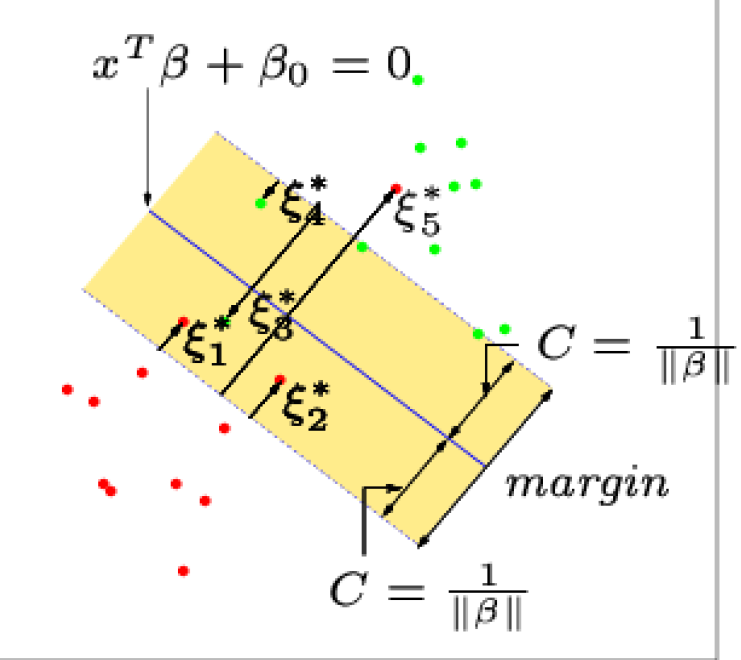
\includegraphics[width=\columnwidth]{media/image33.png}

\textbf{50. Describe the notion of margin in kernel methods.}

Suppose we have two class data, that can be separated with a straight
line. We would like all the points to be as far from the line as
possible (and on the correct side).

C is the minimum distance between each point and the separating line.
\textbf{C= 1/ \textbar b\textbar{}} where b's are the parameter of the
model. Margin is the area around the separating line that has width of
2C. We do not want points inside the margin. This is why we tune C such
that the sum of all errors * 1/C will be smaller than some con7stant.

\textbf{51. What is the purpose of different kernels (linear,
polynomial, RBF) in SVM?}

\textit{Linear:} trivial

\textit{Polynomial}: we allow SVM to produce a non-linear decision
boundary.

\textit{Radial basis function (RBF):}

\[ K(x, x') = \exp \left( - \frac{ | x - x' | ^2 }{ 2\sigma^2} \right) \]

Euclidean distance divided by a free parameter $\sigma^2$

Since the value of the RBF kernel decreases with distance and ranges
between zero (in the limit) and one (when $x = x'$), it has a ready
interpretation as a \textit{similarity measure}

\textbf{52. Describe how to use SVM for more than two classes?}

\textit{One versus All}: build k different models (k=number of
classes) and classify an example to the class that gives highest
probability.\\
\textit{One versus One}: fit (k 2) models (every possible pair) and
classify to the class that wins most pairwise competitions.

Choose 1v1 if k is small enough.

\textbf{53. Describe different activation functions in neural networks
(NNs).}

Activation functions are mathematical equations that determine the
output of a neural network.

\textit{Step functions:} $f(x) = {1 \text{ if } x > 0 \text{ else } 0}$

\textit{ReLU (Rectified Linear Unit):} $f(x) = \max(0, x)$

\textit{Sigmoid function} $ S(x) = 1/(1+\exp(-x)) $

\textit{Softplus:} $f(x) = \ln(1+e^x)$ (\textit{approximation of ReLU})

\textbf{54. Describe the main idea of backpropagation learning for NNs.}

\begin{itemize}
\item Initialize the weights to small random numbers, associated with biases.
\item Propagate the inputs forward (using activation functions)
\item Backpropagate the error (by updating the weights and biases)
\end{itemize}

\textbf{55. Describe the role of criterion (loss) function in
NN?}
\[C = -\sum_j t_j \log y_j \]
\[ \frac{\partial C}{\partial z_i} = \sum_j\frac{\partial C}{\partial y_j} \frac{\partial y_j}{\partial z_i} = y_i - t_i \]
Where $t_i$ is the target and $y_i$ predicted value.

To see how much we missed in classifying an input. We use this to
backpropagate and improve the network.

If we have a scalar output, we use criterion function to see where we
made mistakes. We frequently use cross entropy as cost function C.

\textbf{56. Describe the strengths and weaknesses of NN?}

\textit{Weaknesses:} long training time, require a number of
parameters determined empirically, poor interpretability, overfitting is
a usual, gradient based BP we have no guarantee of reaching the global
optimum.

\textit{Strengths:} high tolerance to noisy data, ability to classify
untrained patterns, well suited for continuous valued inputs and
outputs, algorithms are inherently parallel, successful on an array of
real-world data. Can closely approximate any function.

\textbf{57. Describe a few techniques for overfitting prevention in
NNs.}

\textit{Weight decay}: over time if weights haven't been updated in a
while, slowly decrement them and set them to 0.

\textit{Weight sharin}g: not all connections have unique weights,
they are shared among connections.

\textit{Early stopping:} stop before we reach a too high
classification accuracy. Need a separate evaluation set.

\textit{Model averaging}: train multiple models and average the
weights to use on the final model. ``Ensembling'' (not a good option
-\textgreater{} even 1 NN takes a lot of time to train)

\textit{Drop out:} randomly (with some probability) drop a node, when
training.

\textit{Generative pre-training:} \ldots{}

\textit{Bayesian fitting:} not useable, too slow, complex

\textbf{58. What are deep neural networks? What are their main strengths
and weaknesses?}

Deep neural networks are NNs with more than one hidden layer. They
perform \textit{nonlinear regression} (from a statistical point of view).

STRENGTHS: very powerful, high tolerance to noisy data, ability to
classify untrained patterns, well suited for continuous valued inputs
and outputs, algorithms are inherently parallel, successful on an array
of real-world data

WEAKNESSES: long training time, poor interpretability, overfitting is as
usual, requires a lot of data ...

\textbf{59. What are the recurrent networks?}

Is a NN where neurons are also connected backwards (backwards
connections between neurons). One's output is the input back to it's
parent(s).

Used in the text/signal/image processing. Learning is harder, unreliable
gradients, they disappear faster. They are getting ``dropped''.

\textbf{60. Describe the convolutional neural networks (CNN).}

A class of deep NN, most commonly applied to analyzing visual imagery
and language.

CNN were inspired by biological processes in that the connectivity
between neurons resembles the organization of the animal visual cortex.

Idea: many copies of small detectors used all over the image.

It uses pooling and convolution. They learn filters/detectors and
combinations to recognize some items (dots, edges, for example).

Not fully connected -\textgreater{} lighter model

\textbf{61. Describe different components of CNNs.}

\textit{Convolutional layer:} The convolutional layer consists of a
set of filters. (Each filter covers a spatially small portion of the
input data). The network will learn filters that activate when they see
some specific type of feature at some spatial position in the input.

Convolving the filter == dot product between filter and the input.

On this layer we have local connectivity and shared weights.

\textit{Pooling layer:} Progressively reduce the spatial size of the
representation to reduce the amount of parameters and computation in the
network. Speeds up learning and reduces overfitting.

Pooling partitions the input image into a set of non overlapping
rectangles and, for each such sub region, outputs the maximum (minimum
or average) value of the features in that region.

Problem: after several layers we lose the information about the exact
location of the recognized pattern. E.g. nose on the forehead.

\textbf{62. What are the advantages and disadvantages of CNNs?}

\textit{Advantages:} automatically detects important features without
human supervision, lighter model (not fully connected layers
-\textgreater{} less weights), free translation of variance, fewer
parameters take less space -\textgreater{} can be computed in a memory
of a GPU (or across CPUs).

\textit{Disadvantages:} high computational cost, need a lot of
training data!

\textbf{63. What is 1d and 2d convolution?}

1d is convolution over 1 dimension and is used for convolution on words,
characters, lemmas,..

2d is convolution over 2 dimensions and is used for convolution on
images/ text classification.

\textbf{64. Describe the main idea and components of autoencoders?}

Autoencoders are designed to reproduce their input (especially for
images). They compress input into a \textit{latent-space} of usually
smaller dimension. Then they reconstruct the input from the latent space
(even without the noise).

Encoder: compress input into a \textit{latent space} of usually smaller
dimension. h = f(x)

Decoder: reconstruct input from the latent space. r = g(f(x)) with r as
close to x as possible

\textbf{65. What is denoising an autoencoder?}

Get a clean image as input, apply some noise to it and train the
autoencoder to reproduce the clean image.

\textbf{66. Describe the main idea and components of the generative
adversarial networks?}

Two neural networks contest with each other in a game (in the form of a
zero sum game). Use one neural network to generate data for the second
neural network to use as input and have the first NN try to ``fool'' the
second one into mis-classifying the input.

Generator: generate fake samples, tries to fool the Discriminator

Discriminator: tries to distinguish between real and fake samples

Training means improving G and D.

\textbf{67. Describe different inference methods for predictive
methods.}

15.

\textbf{68. Describe different techniques for the explanation of
predictions.}

(( this one might be wrong, not sure ))

\textit{Domain level:} try to explain the ``true causes and
effects''. Usually unreachable except for artificial problems with known
relations (if we can test it with result functions).

Not applicable especially in medicine, business...

\textit{Model-based:} Make the prediction process of a particular
model transparent. Better models enable better explanation at the domain
level.

\textit{Instance-level:} explain predictions for each instance
separately (model-based). \textit{Nomograms}

(For titanic, we would have a separate nomogram for each person. We
average them at the end)

\textit{Model-level:} the overall picture of a problem the model
conveys (model-based). Averaged instance-level models.

\textit{Model agnostic:} Can be applied to any model. change one
input to our black box and see if the output changes significantly. This
means that that input is important. (perturbation-based explanation).

Won't work well for images. For that we use:

\textit{Model-specific explanation technique}

\textit{Method EXPLAIN}: Hide one attribute at a time.

Weakness: there might be 2 attributes needed to be absent at the same
time to see the importance of the 3rd.

\textbf{69. What is the role of clustering in interpretability?}

Clustering is useful in supervised tasks to get insight into the
relation between predicted values Y and basic groups in the data.

\textbf{70. Describe the main idea of perturbation-based explanation
methods?}

Importance of a feature or a group of features in a specific model can
be estimated by simulating lack of knowledge about the values of the
feature or randomly shuffling them to test its importance

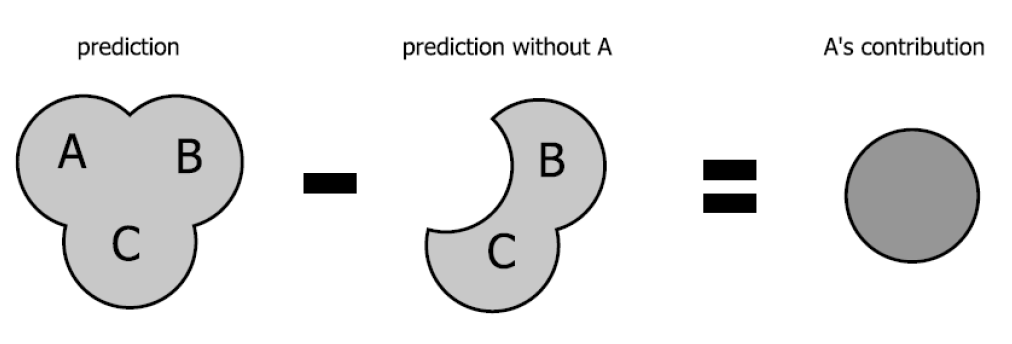
\includegraphics[width=\columnwidth]{media/image6.png}

\textbf{71. Explain the difference between instance-based and
model-based explanations?}

Model based tries to paint the whole picture, while instance based only
explains the instances separately

\textit{Model based}: Make the prediction process transparent of a
particular model. Explanation is independent of the accuracy of a model.
← this is what knowledge extractors are interested in (the overall
picture of a problem the model conveys).

\textit{Instance based}: Explain predictions for each instance
separately (presentation format: impact of each feature on the
prediction value). ← this is what practitioners applying models are
interested in.

\textbf{72. Explain the main idea of the IME, LIME, and SHAP explanation
technique?}

\textit{IME:} Interactions-based Method for Explanation, the feature
gets some credit for standalone contributions and for contributions in
interactions
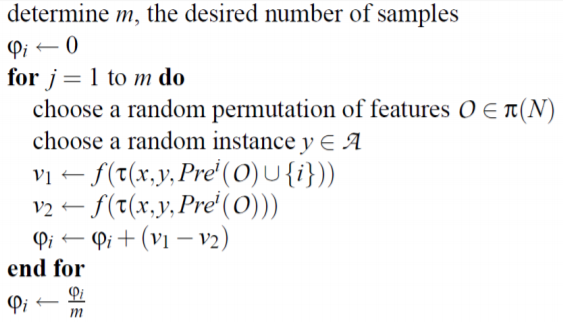
\includegraphics[width=\columnwidth]{media/image21.png}

\begin{itemize}
\item Alternative formulation of \textit{shapley value}
\item ``hide'' any subset of attributes at a time (2 a subsets!)
\item the feature gets some credit for standalone contributions and for contributions in interactions
\end{itemize}

\textit{LIME:} Local Interpretable Model-agnostic Explanations,
perturbations in the locality of an explained
instance.
% 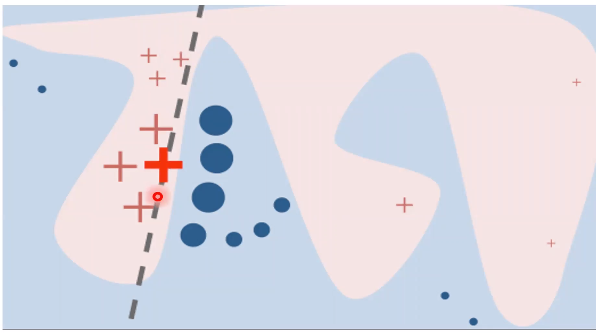
\includegraphics[width=\columnwidth]{media/image25.png}

\begin{itemize}
\item Faster than IME, works for many features (text and images)
\item No guarantees that the explanations are faithful and stable.
\item Neighborhood based: curse of dimensionality
\item may not detect interactions due to simple interpretable local model (linear)
\end{itemize}

\textit{SHAP:} SHapley Additive exPlanation, unification of several
explanation methods, including IME and LIME

(faster than IME but still uses linear model with all its strengths and
weaknesses)

\hypertarget{natural-language-processing-nlp}{%
\section{\texorpdfstring{\textit{Natural language processing
(NLP)}}{Natural language processing (NLP)}}\label{natural-language-processing-nlp}}

\textbf{73. What is the Turing test?}

The turing test is a test where a human is communicating with two other
agents over a computer, one of them another human, the other an AI. The
test tests, if the AI is smart enough to fool the human communicating
with it, that it is also human.

\textbf{74. What is the micro-world approach to NLP?}

Create a ``world'' out of data to analyze. Most text data cannot be
directly processed, so we have to create our own world, where we can
process data.

\textbf{75. Describe the stages of linguistic analysis?}

\textit{Prosody:} the patterns of stress and intonation in a language

\textit{Phonology}: systems of sounds and relationships among the
speech sounds that constitute the fundamental components of a language

\textit{Morphology}: the amissible arrangement of sounds in words:
how to form words, prefixes and suffixes

\textit{Syntax}: the arrangement of words and phrases to create
well-formed sentences in a language

\textit{Semantics}: the meaning of a word, phrase, sentence or text

\textit{Pragmatics}: language in use and the context in which it is
used, including such matters as deixis, taking turns in conversation,
text organization, presupposition and implicature

\textit{Knowing the world}: knowledge of the physical world, humans,
society, intentions in communications

\textbf{76. Describe how to preprocess text in text mining.}
To lower case, Remove punctuation, Remove numbers, Remove stopwords (a, and, the, of,...), Strip whitespaces, Stem the text

\textbf{77. Describe lemmatization, stemming, POS tagging, dependency
parsing, and named entity recognition.}

\textit{Lemmatization}: the process of grouping together the
different inflected forms of a word so they can be analyzed as a single item

\textit{Stemming}: reduce the words to their root ``state'' (it is
getting out of use.)

\textit{POS tagging}: assigning the correct part of speech (noun,
verb, subject, object,...) to words

\textit{Named entity recognition:} seeks to locate and classify named
entities mentioned in unstructured text into predefined categories such
as person names, organizations, locations, medical codes,...

\textit{Dependency parsing}: find connections (dependencies) between
words

\textbf{78. Describe the basic language resources for English and
Slovene (or your language).}

Corpora, wiki, SSKJ, FRAN, GigaFida, KRES, ccKres, GOS, JANES, KAS

\textbf{79. Describe the structure of WordNets.}

WordNet is a database composed of synsets (cognitive synonyms):
Synonyms, Hypernyms, Hyponyms, Meronyms, Holonyms, Etc.

WordNet® is a large lexical database of English. Nouns, verbs,
adjectives and adverbs are grouped into sets of cognitive synonyms
(synsets), each expressing a distinct concept. Synsets are interlinked
by means of conceptual-semantic and lexical relations.

\textbf{80. Describe approaches to document retrieval.}

Historically people \textit{used keywords,} but \textit{today
\textit{full text search}} is used (by the help of organized databases,
indexing and good searching algorithms)

\textbf{81. Describe the inverted file index.}

Is a data structure that maps words to documents.

Inverted file index means that we have a database where for every word
we store in how many documents it appeared and the overall number of
appearances. Then it has a pointer to the document where we can find the
location of the word in the document.

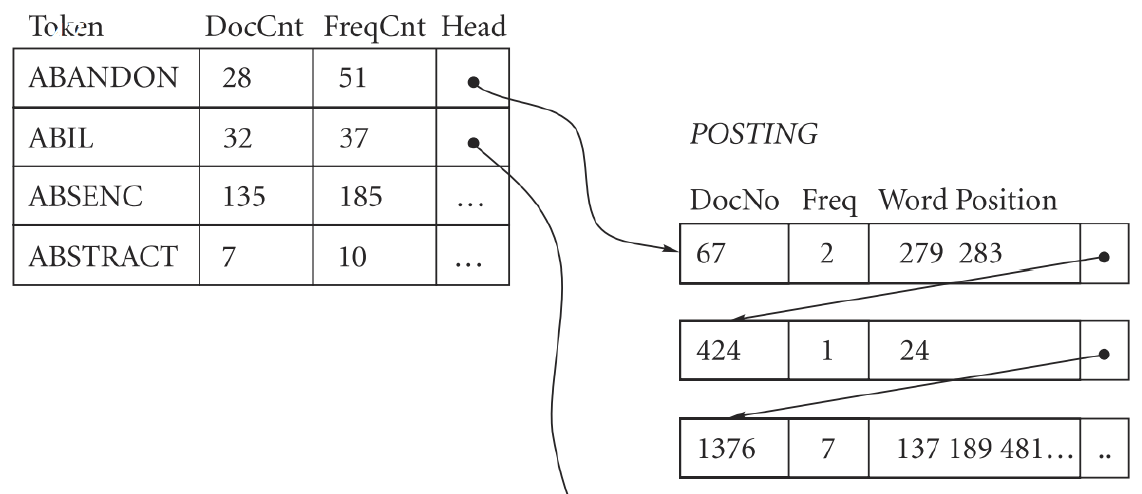
\includegraphics[width=\columnwidth]{media/image10.png}

\textbf{82. Compare search with logical operators and ranking based
search.}

Search with \textit{logical operators} is outdated. It returns a lot
of results, we need to write large queries, synonyms are a problem,
there is no partial matching and no weighting.

\textit{Ranking based search} is used nowadays for web search (Yahoo,
Google, Bing, ...). Less frequent terms are more informative. It uses
vector based representation of documents and queries. For ranking based
search we can explain what bag-of-words approach is or dense embeddings.

\textbf{83. Describe one-hot-encoding and bag-of-words representation.}

\textit{One-hot-encoding} is the vector representation that consists
of only 1 bit set to 1 and all other bits to 0. It assures that machine
learning does not assume that higher numbers are more important.

\textit{Bag of words} representation is commonly used in NLP, where a
text or a document is represented as the bag of its words and how many
times every word appears.

\textbf{84. Describe how to use term-document and term-term matrix?}

\textit{Term-document matrix} is the matrix where every line is one
term and the columns are the documents. Every cell of the matrix shows
how many times some term appeared in a document. This matrix is used for
\textbf{comparison of terms}.

\textit{Document-term matrix} is the other way around, (basically
transposed TDM) and it is used for \textbf{comparison of documents}.

\textit{Term-term} matrix is a matrix where every line is one term
and every column is one term. If two terms appear together more often
they have a higher score in the matrix.

\textbf{85. What is word embedding? Which embeddings are sparse and
which are dense?}

Word Embeddings are dense representations of the individual words in a
text, taking into account the context and other surrounding words that
that individual word occurs with.

\textit{Sparse embeddings:} SVD

\textit{Dense embeddings} are the ones that have less dimension, less
space, they capture synonyms better, and reduce noise. We use LSA
(latent semantic analysis) for truncating the matrices with eigenvalues.

\textbf{86. Describe the use of cosine similarity on documents.}

When comparing documents only the angle between their vectors matters,
this is why cosine similarity is used.

\textbf{87. Describe TF-IDF weighting.}

Inverse document frequency (idf) is equal to:

N - number of documents in collection

Nb - number of documents with word b

IDFb = log(N/Nb) (lower value == more distinct term. If Idf = 0, then
this term is present in every document)

Weight of word b in document d would be equal to :

Wbd = TFbd * IDFbd

Where TFbd is frequency of the term b in document d

\textbf{88. Describe precision, recall, and F1 measures in document retrieval.}

\textit{Precision}: proportion of relevant documents in the obtained ones

\textit{Recall}: proportion of obtained relevant documents. How many
of the relevant documents we succeeded retrieving.

F1 is just weighted harmonic mean (where beta = 1), weighted precision
and recall

\[ F1 = \frac{2 \cdot \text{precision} \cdot \text{recall} }{\text{precision} + \text{recall}} \]

\textbf{89. Describe problems of web search and possible improvements.}

Problems

\begin{enumerate}
\def\labelenumi{\arabic{enumi}.}
\item No content control
\item Different quality of documents
\item Up-to-date?
\item (in)valid links
\item Search engine manipulation (link farms)
\end{enumerate}

Improvements:

\begin{enumerate}
\def\labelenumi{\arabic{enumi}.}
\item Use dictionary, thesaurus (a book that lists words in groups of
  synonyms and related concepts), synonyms
\item Query expansion with relevance information (user feedback,
  personalization, trusted document sources)
\item Semantic search
\item Specific types of queries require specific approaches
\item Trustful sources - Wikipedia
\item Hubs with relevant links
\item Graph theory and analysis
\item Additional information: titles, meta-information, URL
\item Ranking of documents based on links
\end{enumerate}

\textbf{90. Describe the idea of the PageRank algorithm and its possible uses.}

Page rank algorithm determines the rank of a page based on the quality
and number of pages pointing to it

Possible uses: was used by google to order search results

\begin{align*}
  p \quad &\dots \quad \text{web page} \\
  O(p) \quad &\dots \quad \text{pages pointed to by $p$} \\
  I(p) = \{i_1, \dots, i_n\} \quad &\dots \quad \text{pages pointing to $p$} \\
  d \in [0, 1] \quad &\dots \quad \text{damping factor, usually $\approx 0.85$} \\
  \pi(p) \quad &\dots \quad \text{page quality} \\
\end{align*}
\[ \pi(p) = (1-d) + d\frac{\pi(i_1)}{O(i_1)} + \dots + d\frac{\pi(i_n)}{O(i_n)}\]


\textbf{91. Describe the main ideas and implementation of LSA, word2vec,
ELMo, and BERT.}

\textit{LSA}: uses term-context matrix, the idea being the words with
similar context should be closer. It reduces the dimensionality of the
matrix with SVD and uses k most important dimensions to represent the
embedding of the words. (basically PCA)

\textit{Word2vec}: instead of counting how many times a word appears
near another word. It trains a classifier to answer that question (for
example NN). Then it uses classifiers learned weights as the word
embeddings. It doesn't take context into an account. Solution: ELMo and
BERT.

\textit{ELMo}: looks at the entire sentence before assigning each
word in it an embedding. ELMo predicts the next word in a sequence of
words - a task called \textit{Language Modeling (LM)}. first layers
capture morphological and syntactic properties, deeper layers encode
semantical properties.

\textit{BERT}: predicts masked words in a sentence. also predicts
order of sentences: is sentence A followed by sentence B or not \ldots{}
train a classifier built on the top layer foreach task that you fine
tune for , e.g ., Q\&A, NER, inference. achieves state of the art
results for many tasks.

Used form: MLM (masked language model) - delete some words in the
sentence and try to predict them. Needs context of both sides of the
word.

Dominates text classification field.

\textbf{92. Which are the desired properties of word embeddings?}

They shall preserve relations from the original space. We need
\textit{dense vector embeddings}.

\begin{itemize}
\item Matrix based transformations to reduce dimensionality (SVD or LSA -
  latent semantic analysis)
\item Neural embeddings (word2vec, Glove)
\item Contextual neural embeddings (ELMo, BERT)
\end{itemize}

SVM, deep NN -\textgreater{} both require numerical input

1-hot-encoding and a bag of words do not preserve semantic similarity.
:(

\textbf{93. Compare different types of word embeddings.}

\begin{enumerate}
\def\labelenumi{\arabic{enumi}.}
\item Frequency based Embedding (Count vector, TD-IDF, co-occurrence vector)
\item Prediction based Embedding (Continuous Bag of words, Skip -- Gram
  model)
\end{enumerate}

\begin{itemize}
\item Dense vector embeddings
\item Neural embeddings
\item Diachronic embeddings
\item Contextual embeddings
\item Cross-lingual embeddings
\end{itemize}

\textbf{94. Describe a few relations expressed with modern word
embeddings.}

Diachronic embedding: comparing words and their neighbours throughout
history.

\textbf{95. What sort of biases are reflected in word embeddings?}

Cultural biases, usually negative biases

\textbf{96. How to use BERT and multilingual BERT for text
classification?}

train a classifier built on the top layer for each task that you fine
tune for , e.g ., Q\&A, NER, inference.

\begin{itemize}
\item Sentence classification (sentiment, grammar\ldots)
\item Two sentence classification
\item Questions/answers
\end{itemize}


\textbf{97. Describe the idea and a few uses of cross-lingual
embeddings?}

Word clouds of different languages can be aligned.

\begin{itemize}
\item transfer between languages: models, resources
\item embedded words enter neural networks
\item replace them with cross lingual embeddings and easily switch languages
\end{itemize}

\textbf{98. Describe a few semantic technologies and a few important NLP
tasks.}

\textit{Semantic technologies aka Text mining:} to acquire new
knowledge. Summarization, document relations, clustering of documents,
related news, new topic detection, q\&a, named entity recognition,
inference, coreference resolution.

\textit{NLP tasks:} document retrieval, information extraction, document 
classification, document summarization, sentiment analysis, text mining, 
machine translation, language generation

\textbf{99. How to approach text summarization, sentiment
classification, machine translation (MT), or question answering
problems?}

\textit{Text summarization}: general, guided (describe in advance
what sort of information do you want). One/multi document. Extractive
and abstractive (mix 2 words like increase/decrease).

For short text we use \textit{abstractive} summarization.

For longer texts we use \textit{extractive} summarization.

\textit{Sentiment classification:}

Binary, tenary, n-ary

We use lexicon of positive/negative words

Machine learning based.

MT:

With BERT, RNN, Encoder-Decoders, NMT(neural machine translation)

\textbf{100. What are the language model and translation model in MT?}

\textit{Language model:} each target (English) sentence e is assigned
a probability p(e). Estimation of probabilities for the whole sentences
is not possible (why?), therefore we use language models, e.g., 3 gram
models or neural language models.

\textit{Translation model:} We have to assign a probability of p(
f\textbar e ), which is a probability of a foreign language sentence f,
given target sentence e. We search the e which maximizes p(e) *
p(f\textbar e). We take into account the position of a word and how many
words are needed to translate a given word.

Noisy channel: given sentence e, we transmit it through noisy channel
and get a corrupted sentence f. For reconstruction we need 1) how to
speak original language (language model p(e)) and 2) how to transform f
into e (translation model, p(f\textbar e))

\textbf{101. What is the encoder-decoder model in NLP?}

\textit{Encoder}: use word representation → word , 1 hot vector,
dense embedding, recurrent network

\textit{Decoder:} computation of the next state of recurrent network,
probability of the next word, selection of the next word

Encoder takes a sentence and transforms it into latent vector
representation. Decoder takes that latent vector representation and
transforms it back into a sentence. Both are language specific.

% 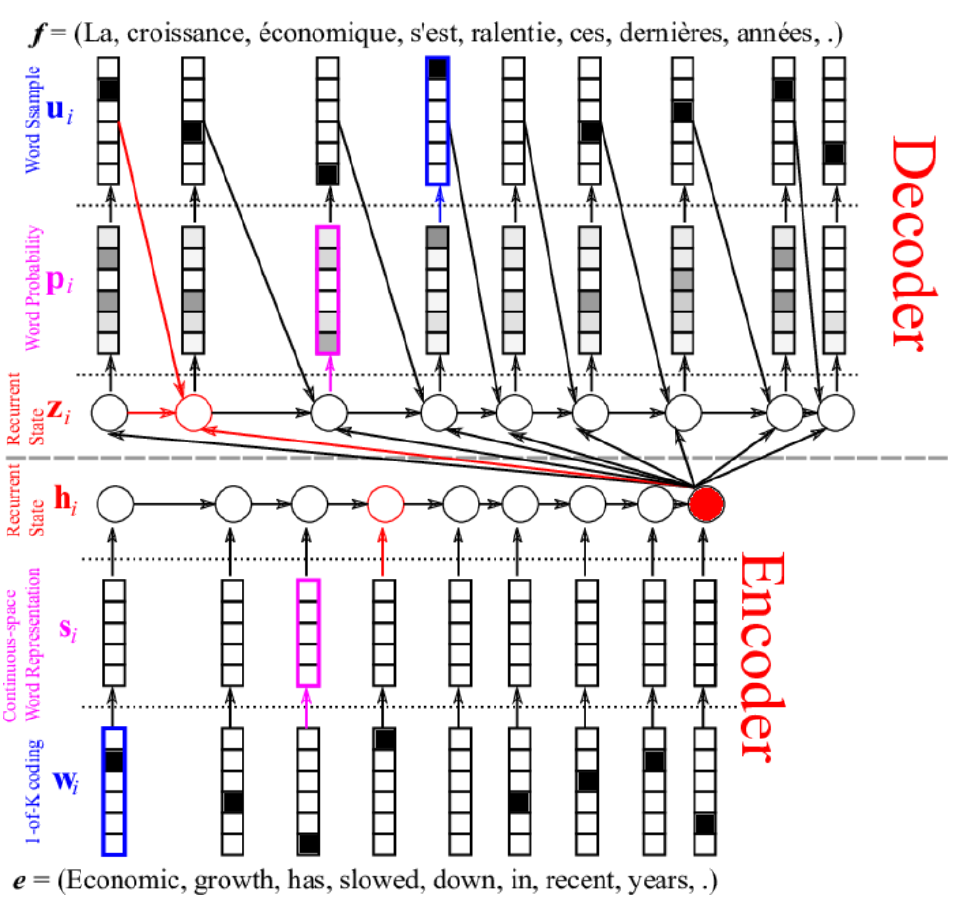
\includegraphics[width=\columnwidth]{media/image40.png}

\textbf{102. What is the attention mechanism in deep neural networks?}

Usually for each word in a sentence a hidden state vector called context
is output from an encoder and this vector is fed back into the input and
not into the decoder until the end of sentence is detected, then decoder
produces output one step at a time. This is problematic for long
sentences, this is where the attention mechanism comes in which produces
a special context vector for each decoder time step.

\section{Reinforcement learning}

\textbf{103. Describe when and why to apply RL.}

We can use it when we are in an environment where we can afford to make
mistakes. When we need to make decisions in \textit{an uncertain
environment.}

Why?: simple algorithms, works most of the time, no need to label the
data (it takes a lot of time, money or it is just hard to - label
regions of objects in 15 million images).

\textbf{104. What are the differences between supervised learning and
RL?}

You don't get examples of correct answers, you have to try things in
order to learn.

\textbf{105. Describe the explore or exploit dilemma in RL?}

We can't always choose the action with the highest Q-value. The
Q-function is initially unreliable, we need to explore until it is
optimal.

Explore: gather information from environment

Exploit: use information to make better decision

\textbf{106. Describe the four main components of RL and their role.}

\begin{enumerate}
\def\labelenumi{\arabic{enumi}.}
\item Policy: defines agents choices and actions in a given time
\item Reward: feedback from the environment. Agent tries to maximize it
\item Value: agents expectation of what can be expected in a given state (it
  predicts rewards)
\item Model: internal representation of environment
\end{enumerate}

\textbf{107. How the interface between the agent and environment works
in RL?}

Agents and the environment interact at discrete time steps. Agent
observes state $s(t)$ at step $t$ and produces an action $a(t)$,
giving a resulting reward $r(t + 1)$ and next state $s(t + 1)$.

\textbf{108. Describe returns for episodic and continuing tasks.}

\textit{Episodic}: interaction breaks naturally into episodes (eg.
plays of a game, trips through a maze)

\textit{Continuing}: interaction does not have natural episodes.

IN OTHER WORDS ...

Episodic tasks are the tasks that have a terminal state (end). In RL,
episodes are considered agent-environment interactions from initial to
final states. For example, in a car racing video game, you start the
game (initial state) and play the game until it is over (final state).
This is called an episode. Once the game is over, you start the next
episode by restarting the game, and you will begin from the initial
state irrespective of the position you were in the previous game. So,
each episode is independent of the other.

In a continuous task, there is not a terminal state. Continuous tasks
will never end. For example, a personal assistance robot does not have a
terminal state.

\textbf{109. What is the discounted return, and what is its role?}

\[ R_t = r_{i+1} + \gamma r_{i+2} + \gamma^2 r_{i+3} + \dots = \sum_{k=0}^\infty \gamma^k r_{i+k+1}\]

where $\gamma \in [0,1]$ is the \textit{discount rate} it makes rewards 
further in the future lass valuable.

\textbf{110. What is the average reward model, and what are its
advantages and disadvantages?}

It's a model where the agent optimizes long-term average reward. The
downside is that it does not know the difference between near and
distant rewards

\textbf{111. What is the role of Markov property in RL?}

If a state summarizes all past sensations so as to retain all
``essential'' information it has the Markov property.

Used in MDP (Markov decision process) and Bellman Optimality Equation.\\
~\\
Markov property is that the next decision is solely dependent on the
current state. All of the states before this one are meaningless for the
next decision.

\textbf{112. Describe the Markov decision problem (MDP).}

If a task has the Markov property, it is basically a Markov Decision
Process. If state and action sets are finite, it is a finite MDP. To
define a finite MDP we need:

\begin{itemize}
\item State and action sets
\item One step ``dynamics'' defined by transition probabilities
\item Reward probabilities
\end{itemize}

\textbf{113. What sort of learning simplifications does MDP allow in
RL?}

MDP can be solved by linear programming or by a dynamic programming
method. MDP is a discrete, stochastic and controlled process. At any
given time, the process is in a certain 's' state, and the user can
select any 'a' action that is available in the 's' state. The process
responds to this action at the next time unit by random moving to a new
state s' and giving the user a corresponding reward.

\textbf{114. Describe the State-value function and action-value
functions?}

\textit{State-value function:} $V^\pi(s)$ returnes the expected
revard starting from the state $s$ using policy $\pi$
\[ V^\pi (s) = E_\pi \{ G_t | s_t = s \}\]
where $G_t$ is total discounted reward from time step $t$.

\textit{Action-value function:} $Q^\pi (s, a)$ returnes the expected revard
of taking an action $a$ in a state $s$ under policy $\pi$.

\[ Q^\pi (s, a) = E_\pi \{ G_t | s_t = s, a_t = a\}\]

The relationship between $Q$ and $V$:
\[ V^\pi(s) = \sum_{a \in A} \pi(a | s) Q^\pi (s,a)\]


\textbf{115. Describe the Bellman equations and their role in RL?}

Bellman eq. give us the ability to calculate all the expected rewards in
all states. It is basically n equations with n variables. If we solve
them we get an optimal reward for every state we are in. This is how we
do RL ...

\textbf{116. What is the role of the optimal value function and optimal
action-value function?}

For finite MDP's policies, they can be partially ordered:

\[ \pi \geq \pi' \quad \iff \quad \forall s \in S : \ V^\pi (s) \geq V^{\pi'}(s)\]

This means that there are always one or more policies that are better or
equal to all the others. These are optimal policies. Optimal policies
share the same state-value function and action-value function.

\begin{align*}
  V^*(s) &= \max_\pi V^\pi (s) \quad \forall s \in S \\
  Q^*(s, a) &= \max_\pi Q^\pi (s, a) \quad \forall s \in S, a \in A(s)
\end{align*}
  
Basically the optimal value function and the optimal action-value
function return the expected return (reward) for following the optimal
policy. This also means that they tell us what the optimal action in a
state is.

\textbf{117. How can we get the optimal policy from the optimal
action-value function?}

The value of a state under an optimal policy must equal the expected
return for the best action from that state

\begin{align*}
  Q^*(s,a) &= E \left\{ r_{t+1} + \gamma \max_{a'} Q^* (s_{t+1}, a') | s_t = s, a_t = a \right\} \\
   &= \sum_{s'} P_{ss'}^{a} \left[ R_{ss'}^a + \gamma \max_{a'} Q^*(s', a')\right]
\end{align*}

$Q$ is the unique solution of this \textit{system of nonlinear equations}.
Once we have $Q^*$ we can further calculate the optimal policy by taking
the optimal action:

\[ \pi^*(s) = \underset{a \in A(s)}{\text{argmax}}\ Q^*(s,a)\]

\textbf{118. How to solve Bellman optimality equations?}

Finding an optimal policy by solving the Bellman optimality equation
requires the following:

\begin{itemize}
\item accurate knowledge of environment dynamics;
\item enough space and time to do the computation;
\item the Markov property must be true.
\end{itemize}

\^{} can be done with dynamic programming

We usually have to settle for approximations → Monte Carlo, Value
Iteration, Q-learning

\textbf{119. When and how dynamic programming is used in RL?}

We need a complete model of the environment and rewards (state space,
action space, transition model).

Idea: start with any policy, then iteratively improve it (calculate
V(policy), then improve policy based on that V(policy))

\textbf{120. Describe policy-value iteration, value iteration, and
policy iteration approaches to RL?}

\textit{Policy iteration}: $V(\pi_0) \to \pi_1,\ V(\pi_1) \to \pi_2,\ \dots$ \\
$V(\pi_i)$ doesn't need to converge, just move towards the best one

\textit{Value iteration}:
\[ V_{k+1} (s) = \max_a \sum_{s'} P_{ss'}^a \left[ r_{ss'}^a + \gamma V_k(s') \right]\]

\begin{itemize}
\item use Bellman optimality equation as an update
\item Converges to $V^*$
\end{itemize}

\textbf{121. Describe the convergence criterion for value iteration.}

If the maximum difference between two successive value functions is less
than $\varepsilon$, then the value of the greedy policy, (the policy obtained by
choosing, in every state, the action that maximizes the estimated
discounted reward, using the current estimate of the value function)
differs from the value function of the optimal policy by no more than 
$2\varepsilon \lambda/(1-\lambda )$ at any state. This is an effective stopping 
criterion for the algorithm

\textbf{122. Describe the Monte Carlo approach to RL and when it is
used.}

We use Monte Carlo methods as an approximation for the optimal policy.
We don't need full knowledge of the environment. We only need experience
or simulate experience. This method can only be used for episodic tasks.
The way it works is by simulating a few paths and then averages all the
returns. So to estimate V(s) we average all observed returns in state s.

\textbf{123. Describe the $\varepsilon$-greedy policy.}

\begin{itemize}
\item with probability $1-\varepsilon$ perform the optimal/greedy action
\item with probability $\varepsilon$ perform a random action
\item will keep exploring the environment
\item slowly move it towards greedy policy: $\varepsilon \to 0$
\end{itemize}

We use it in Q-learning as an ``explore'' method, because we can't
always choose the action with the highest Q value. (The Q function is
initially unreliable, we need to explore until optimal!)

\textbf{124. Describe learning with time differences (TD) in RL?}

Previous states receive a portion of the difference to successors.
(difficult for analysis)

For $\lambda = 0$:
\[ V(s_t) = V(s_t) + c \cdot \left(V(s_{t+1}) - V(s_t) \right)\]

where $c$ is a parameter, slowly decreasing during learning ensuring convergence

For $\lambda > 0$, more than just immediate successors are taken into account (speed)

\textbf{125. Describe the Q-learning.}

Works with $Q$ function instead of $V$ function.

$Q(s, a)$ estimates the \textbf{discounted cumulative reward} (start in s,
take action a, follow the current policy thereafter)

Suppose we have the optimal $Q$ function → optimal policy is $\text{argmax}_b\ Q(s, b)$

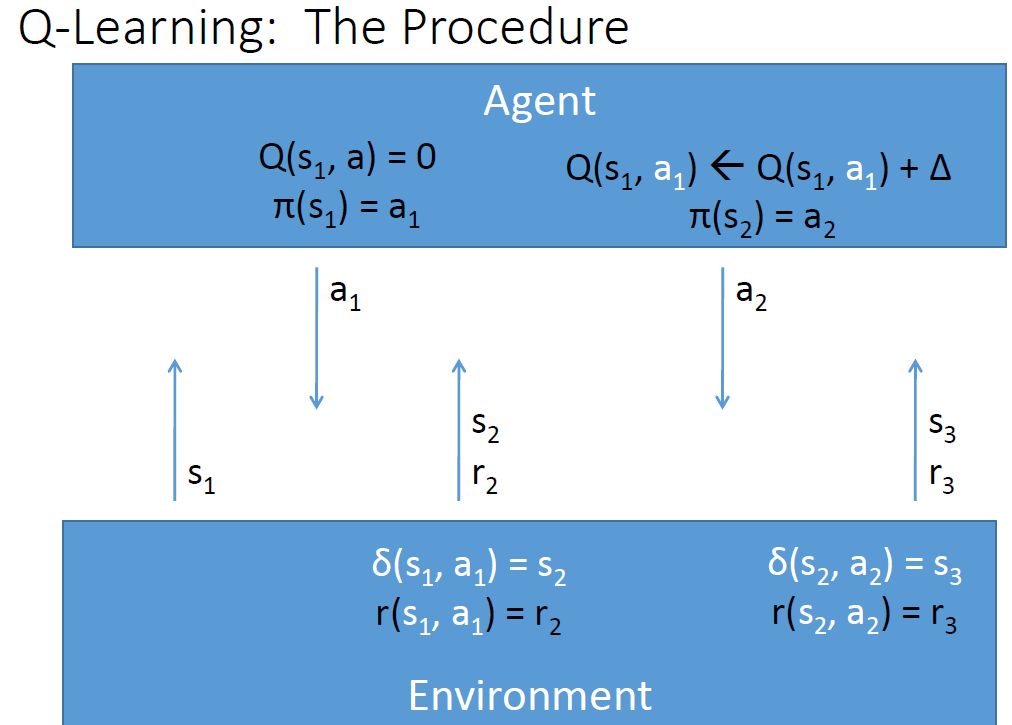
\includegraphics[width=\columnwidth]{media/image3.png}

Pseudo code:

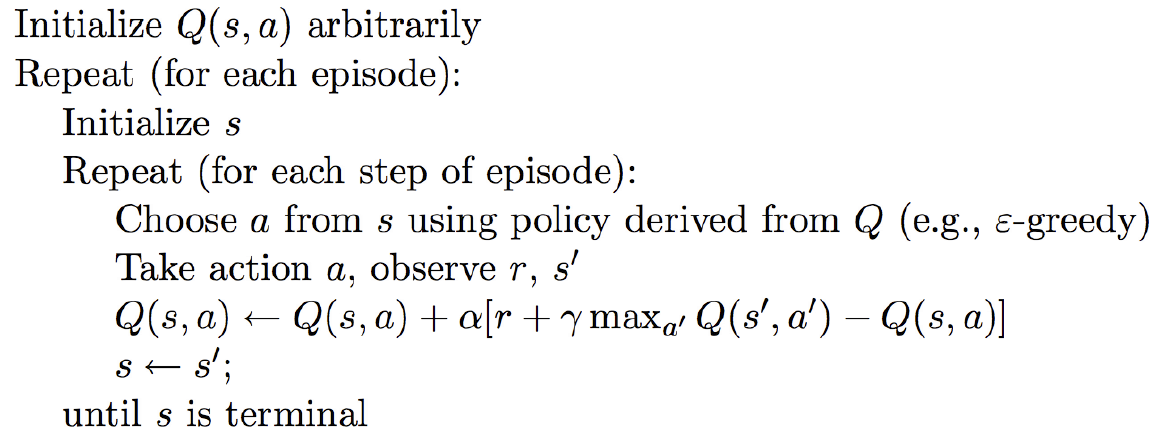
\includegraphics[width=\columnwidth]{media/image14.png}

\textbf{126. What are the updates in Q-learning? How to assure
exploration?}

Q-learning updates:
\begin{itemize}
  \item basic update equation:
  \[ Q(s, a) \leftarrow r(s, a) + \max_b Q(s', b)\]
  \item with a discount factor to give later rewards less impact:
  \[ Q(s, a) \leftarrow r(s, a) + \gamma \max_b Q(s', b)\]
  \item with a learning rate for non-deterministic worlds:
  \[ Q(s, a) \leftarrow \big[ q-\alpha \big] Q(s, a) + \alpha \big[ r(s, a) + \gamma \max_b Q(s', b) \big] \]
\end{itemize}

Assure exploration: $\varepsilon$-greedy!

\textbf{127. How to use function approximation in RL?}

Used when in complex environments (Q is too complex), we describe a
state with a \textit{feature vector}. We can then calculate Q as any
regression model by using the state feature vectors as its parameters.
(\textless-\/- e.g.)

??

\textbf{128. How to measure and compare the learning performance of RL
learners?}

\begin{itemize}
\item \textit{Eventual convergence to optimality (}Many algorithms come
  with a provable guarantee of asymptotic convergence to optimal
  behavior. This is reassuring, but useless\textit{)}
\item \textit{Speed of convergence to optimality} (more practical → speed
  of convergence to near optimality (how near?) OR level of performance
  after a given time (what time?))
\item \textit{Regret} (expected decrease in reward gained due to
  executing the learning algorithm instead of behaving optimally from
  the very beginning; these results are hard to obtain)
\end{itemize}
